\chapter{Introducción}
\label{chap:antecedentes}

Los programas de computador comerciales para el análisis y diseño de estructuras que se encuentran vigentes a la fecha cuentan, en general, con un entorno gráfico que le permite al usuario describir el modelo de forma interactiva, procesarlo y visualizar los resultados de manera conveniente.\\

En \cite{escamilla1995microcomputadores} se presenta una lista de algunos de estos programas de uso común en América Latina, entre los cuales se encuentra \emph{ETABS} (Three Dimensional Analysis of Building Systems - Extended Version).\\

ETABS es un programa de computador creado por Edward Wilson, Jeffery Hollings y Henry Dovey en 1975. Según \cite{ETABS1975}, este programa de computador fue desarrollado para el análisis estructural lineal de edificios de pórticos y muros a cortante sujetos tanto a cargas estáticas como sísmicas. El edificio es idealizado como un sistema de elementos tipo pórticos y muros a cortante independientes interconectado por losas de entrepiso las cuales son rígidas en su propio plano. \\

Este programa es una extensión de \emph{TABS} (Three Dimensional Analysis of  Building Systems) para poder analizar pórticos en tres dimensiones. Según \cite{ETABS1972}, una de las razones para desarrollar TABS fue darle una retroalimentación a los usuarios de los programas \emph{FRMSTC} (Static Load Analysis of High-Rise Buildings), \emph{FRMDYN} (Dynamic Analysis of Multistory Buildings), \emph{LATERAL} y \emph{SOLID SAP} (Static Analysis Program for Three-Dimensional Solid Structures).\\

FRMSTC permitía analizar edificios simétricos con pórticos y muros a cortante paralelos sujetos a cargas estáticas y evaluar los modos y las frecuencias. FRMDYN era similar a FRMSTC con la excepción que la carga era la aceleración del terreno debido a un desplazamiento dependiente del tiempo. LATERAL fue una extensión de FRMSTC que permitía analizar linealmente pórticos y muros a cortante que no eran necesariamente paralelos con tres grados de libertad en cada piso. SOLID SAP era un programa general de elementos finitos y tenía una opción que permitía introducir la aproximación de piso rígido. Este programa también tenía la opción de realizar análisis dinámico.\\

En la actualidad, ETABS se encuentra en la versión 18.1.1 y según \cite{ETABS2020systemrequirements}, puede ser ejecutado en computadores con sistema operativo Windows 7, Windows 8 o Windows 10 con arquitectura de 64 bits que cuenten como mínimo con un procesador Intel Pentium 4 o AMD Athlon 64, una resolución de 1024x768 pixeles con 16 bits por canal, 8 GB de RAM y 6 GB de espacio en el disco duro. En la figura \ref{fig:etabs_start_page} se presenta la ventana del programa ETABS ejecutandose en un computador con Windows 10.\\

\begin{figure}[ht]
    \centering
    \begin{annotationimage}{width=0.5\textwidth}{introduction/etabs-startup.png}
        \draw[annotation left = {{Barra de título} at 0.91}] to (0.15, 0.81);
        \draw[annotation left = {{Barra de menús} at 0.7}] to (0.15, 0.8);
        \draw[annotation left = {{Explorador del modelo} at 0.5}] to (0.18, 0.65);
        \draw[annotation left = {{Barra de herramientas} at 0.3}] to (0.15, 0.4);
        \draw[annotation left = {{Barra de estado} at 0.125}] to (0.15, 0.225);
        \draw[annotation right = {{Barra de herramientas} at 0.655}] to (0.84, 0.765);
        \draw[annotation right = {{Vista del modelo} at 0.47}] to (0.75, 0.67);
        \draw[annotation right = {{Indicador de actualizaciones} at 0.86}] to (0.85, 0.76);
    \end{annotationimage}
    \caption{Ventana del programa ETABS ejecutandose en Windows 10.}
    \label{fig:etabs_start_page}
\end{figure}

A través de múltiples cuadros de diálogo, los cuales son accesibles ya sea a través de la barra de menús, las barras de herramientas, el explorador del modelo, las vistas del modelo o con atajos de teclado, el usuario es capaz de modelar la estructura que desea analizar al describir los materiales, las secciones transversales, los elementos estructurales, las condiciones de apoyo, los diafragmas y las cargas. \\

Según \cite{ETABS2017analysisreferencemanual}, ETABS analiza el modelo usando el motor de análisis \emph{SAPFire}, el cual es común a otros programas de la misma compañia (\emph{SAP2000}, \emph{SAFE} y \emph{CSiBridge}). SAPFire es la última versión de la serie de programas \emph{SAP} y ofrece las siguientes herramientas:
\begin{itemize}
    \item Análisis estático y dinámico,
    \item Análisis lineal y no lineal,
    \item Análisis sísmico y análisis incremental no lineal (\emph{pushover}),
    \item Análisis de cargas móviles,
    \item No linealidad geométrica, incluyendo efectos P-delta y grandes desplazamientos,
    \item Etapas constructivas,
    \item Fluencia lenta (\emph{creep}), retracción (\emph{shrinkage}) y envejecimiento,
    \item Análisis de pandeo,
    \item Análisis de densidad espectral de potencia y estado estacionario,
    \item Elementos tipo pórtico y laminares, incluyendo el comportamiento de vigas, columnas, cerchas, membranas y placas,
    \item Elementos tipo cable y tendón,
    \item Elementos bidimensionales planos y elementos sólidos asimétricos,
    \item Elementos sólidos tridimensionales,
    \item Resortes no lineales y apoyos,
    \item Propiedades de los resortes y apoyos dependientes de la frecuencia,
\end{itemize}

Con los resultados del análisis del modelo, el posprocesador de ETABS puede \emph{diseñar} los elementos estructurales de acuerdo a uno de varios códigos de diseño de diferentes países. ETABS es capaz de diseñar pórticos en acero, pórticos en concreto, vigas compuestas, columnas compuestas, vigas en acero de alma abierta (\emph{steel joist}), muros a cortpante y losas de concreto.\\

Adicionalmente, según \cite{ETABS2019welcome}, ETABS cuenta con la posibilidad de generar dibujos estructurales esquemáticos de las plantas estructurales, de los despieces de vigas, columnas y muros a cortante, y de los detalles de las conexiones de acero.\\

En términos generales, estos programas de computador comerciales cuenta con características similares a las de ETABS. Actualmente, dichos programas están innovando para permitirle al usuario trabajar con modelos \emph{BIM} (Building Information Modeling).\\

\section{Objetivo}

Desarrollar un programa de computador a código abierto para el análisis de estructuras tridimensionales tipo pórtico sometidas a cargas estáticas.\\

Con este trabajo se pretende contribuir al ejercicio libre de la profesión del ingeniero estructural y a la enseñanza del análisis de las estructuras.

\subsection{Objetivos específicos}

\begin{itemize}
\item Desarrollar el ambiente gráfico y la interfaz gráfica de usuario del programa de computador para permitirle al usuario ingresar los datos que describen la estructura, las acciones a las cuales se encuentra sometida y visualizar los resultados del análisis estructural.
\item Desarrollar el módulo de análisis estructural para calcular el desplazamiento de los nudos, el valor de las reacciones y de las fuerzas internas de los elementos de una estructura sometida a cargas estáticas.
\end{itemize}

\section{Metodología}

Se desarrollaron los programas de computador \emph{pyFEM} y \emph{FEM.js}. El primero para analizar estructuras tridimensionales tipo pórtico sometidas a cargas estáticas y el segundo para modelarlas. Esto con el fin que FEM.js pueda ser usado junto con otro programa de computador diferente a pyFEM.\\

Durante el desarrollo de estos programas se utilizó \emph{git} como sistema de control de versiones. Según \cite{chacon2014git}, git es un sistema distribuido de control de versiones que registra los cambios realizados a un conjunto de archivos para coordinar el trabajo entre programadores.\\

Una copia de los repositorios de pyFEM y FEM.js se encuentran en la página de internet \emph{GitHub}, la cual permite alojar proyectos utilizando git. pyFEM está alojado en \url{https://github.com/rvcristiand/pyFEM} mientras que FEM.js está alojado en \url{https://github.com/rvcristiand/FEM.js}.\\

\subsection{pyFEM}

pyFEM fue desarrollado en \emph{Python}. Según \cite{lutz2013python}, Python es un lenguaje de programación interpretado orientado a objetos cuya filosofía hace enfasis en la legibilidad de su código. Los archivos revelantes que componen el repositorio de pyFEM son:
\pagebreak

\dirtree{%
  .1 pyFEM/.
  .2 LICENSE.
  .2 README.md.
  .2 example\_1.json.
  .2 example\_2.json.
  .2 example\_3.json.
  .2 pyFEM/.
  .3 classtools.py.
  .3 core.py.
  .3 primitives.py.
  .2 test/.
  .3 space\_frame.py.
  .3 trusses.py.
}

\bigskip
El archivo \verb|LICENCE| contiene la licencia de pyFEM, la cual se presenta a continuación.

\begin{quotation}
  MIT License\\

  Copyright (c) 2019 pyFEM\\

  Permission is hereby granted, free of charge, to any person obtaining a copy of this software and associated documentation files (the "Software"), to deal in the Software without restriction, including without limitation the rights to use, copy, modify, merge, publish, distribute, sublicense, and/or sell copies of the Software, and to permit persons to whom the Software is furnished to do so, subject to the following conditions:\\
  
  The above copyright notice and this permission notice shall be included in all copies or substantial portions of the Software.\\

  THE SOFTWARE IS PROVIDED ``AS IS'', WITHOUT WARRANTY OF ANY KIND, EXPRESS OR IMPLIED, INCLUDING BUT NOT LIMITED TO THE WARRANTIES OF MERCHANTABILITY, FITNESS FOR A PARTICULAR PURPOSE AND NONINFRINGEMENT. IN NO EVENT SHALL THE AUTHORS OR COPYRIGHT HOLDERS BE LIABLE FOR ANY CLAIM, DAMAGES OR OTHER LIABILITY, WHETHER IN AN ACTION OF CONTRACT, TORT OR OTHERWISE, ARISING FROM, OUT OF OR IN CONNECTION WITH THE SOFTWARE OR THE USE OR OTHER DEALINGS IN THE SOFTWARE.
\end{quotation}

El archivo \verb|README.md| contiene todas las instrucciones necesarias para ejecutar y usar pyFEM.\\

% TODO: hacer el README.md
% Como se instala el programa

Los archivos \verb|example_1.json|, \verb|example_2.json| y \verb|example_3.json| almacenan los modelos de tres de los ejemplos presentados en \cite{escamilla1995microcomputadores} que han sido analizados con pyFEM. La extensión \emph{json} se usa para indicar que los archivos tienen formato \emph{JSON} (de sus siglas en inglés JavaScript Object Notation), el cual es un formato sencillo para el intercambio de datos. El modelo es descrito de tal manera que puede ser interpretado por FEM.js para generar su representación en una escena tridimensional. \\

La carpeta \emph{pyFEM} contiene los archivos \verb|classtools.py|, \verb|core.py| y \verb|primitives.py| los cuales contienen las instrucciones para analizar los modelos. La extensión \emph{py} se usa para indicar que los archivos son programas de Python.\\

En el archivo \verb|classtools.py| se encuentran las \emph{clases} \verb|UniqueInstances| y \verb|AttrDisplay|, la primera para evitar que se creen \emph{objetos} de una misma clase con la misma información y la segunda para generar una representación conveniente de los objetos.\\

En el archivo \verb|primitives.py| se encuentran varias clases, entre ellas \verb|Material|, \verb|Section|, \verb|Joint|, \verb|Frame|, \verb|Support|, \verb|LoadPattern|, etc., las cuales permiten describir los diferentes atributos del modelo.\\

En el archivo \verb|core.py| se encuentra la clase \verb|Structure| la cual permite describir estructuras para ser analizados. Para crear objetos de esta clase se debe llamar la clase indicando los grados de libertad a tener en cuenta. A partir de un objeto de esta clase es posible describir el modelo de la estructura al agregar materiales, secciones transversales, nodos, elemenetos tipo pórtico, apoyos, patrones de carga, cargas en los nodos y cargas distribuidas en los elementos tipo pórtico.\\

En el ejemplo \ref{ej:cercha-plana} se presenta la solución a un ejercicio de \cite{escamilla1995microcomputadores} usando pyFEM.
\pagebreak

\begin{ejemplo}
  \label{ej:cercha-plana}
  Resuelva completamente la cercha mostrada por el método matricial de los desplazamientos. El material es acero estructural con $ E = 2040\; t / cm^2 $. Las áreas están dadas entre paréntesis en $ cm^2 $.\\

    \begin{center}
      \begin{tikzpicture}
        % Points
        \point{1}{0}{0};
        \point{2}{8}{0};
        \point{3}{4}{3};
        \point{4}{4}{0};
        
        \point{p}{4}{-1.3};
        \point{q}{5.05}{3.7875};
        
        \point{1-3}{2}{1.5};
        \point{1-4}{2}{0};
        \point{3-2}{6}{1.5};
        \point{4-2}{6}{0};
        \point{4-3}{4}{1.5};
        
        % Beams
        \beam{2}{1}{3}[0][0];
        \beam{2}{1}{4}[1][1];
        \beam{2}{3}{2}[1][1];
        \beam{2}{4}{2}[1][1];
        \beam{2}{4}{3}[1][1];
        
        % Supports
        \support{1}{1};
        \support{2}{2};
        
        % Joints
        \hinge{1}{1};
        \hinge{1}{2};
        \hinge{1}{3};
        \hinge{1}{4};
        
        % Loads
        \load{1}{q}[216.87];
        \load{1}{p}[90];
        
        % notation
        \notation{1}{1}{1}[above left];
        \notation{1}{2}{2}[above right];
        \notation{1}{3}{3}[above left];
        \notation{1}{4}{4}[below left];
        
        \notation{1}{3}{$ \SI{5}{\tonne} $}[above right=10mm];
        \notation{1}{4}{$ \SI{20}{\tonne} $}[below right=5mm and 0mm];
        
        \notation{5}{1}{3}[$ (100) $ ][.5][above][0.5];
        \notation{5}{1}{4}[$ (40) $ ][.5][above][0.5];
        \notation{5}{3}{2}[$ (150) $ ][.5][above][0.5];
        \notation{5}{4}{2}[$ (40) $ ][.5][above][0.5];
        \notation{5}{4}{3}[$ (30) $ ][.5][right][1];
        
        
        % Dimensions
        \dimensioning{1}{1}{4}{-1.5}[$ \SI{4}{m} $];
        \dimensioning{1}{4}{2}{-1.5}[$ \SI{4}{m} $];
        \dimensioning{2}{2}{3}{9}[$ \SI{3}{m} $];
      \end{tikzpicture}
      \captionof{figure}{Cercha simple plana del \textit{Ejemplo 7.1} de \cite{escamilla1995microcomputadores}.}
    \end{center}

    \textit{\textbf{Solución -}} En el algoritmo \ref{alg:cercha_plana} se presenta un programa de Python para solucionar el modelo de la estructura usando pyFEM. Las instrucciones consisten en crear un nuevo objeto tipo \verb|Structure|, al cual se le ha dado el nombre de \emph{structure} y, seguidamente, se agregan los materiales, las secciones, los nodos, los elementos tipo cercha, los apoyos, los patrones de carga y las cargas en los nodos. Una vez los datos del modelo de la estructura han sido ingresados, se puede solucionar el modelo mediante la instrucción \verb|structure.solve()|. \\

\begin{lstlisting}[language=Python,caption=Ingreso de los datos del modelo de la estructura a \textit{pyFEM}.,label=alg:cercha_plana, frame=single]
# create the model
model = Structure(ux=True, uy=True)

# add materials
model.add_material(key='1', modulus_elasticity=2040e4)

# add sections
model.add_section(key='1', area=030e-4)
model.add_section('2', area=040e-4)
model.add_section('3', area=100e-4)
model.add_section('4', area=150e-4)

# add joints
model.add_joint(key=1, x=0, y=0)
model.add_joint(2, 8, 0)
model.add_joint(3, 4, 3)
model.add_joint(4, 4, 0)

# add frames
model.add_frame(key='1-3', key_joint_j=1, key_joint_k=3, key_material='1', key_section='3')
model.add_frame('1-4', 1, 4, '1', '2')
model.add_frame('3-2', 3, 2, '1', '4')
model.add_frame('4-2', 4, 2, '1', '2')
model.add_frame('4-3', 4, 3, '1', '1')

# add supports
model.add_support(key_joint=1, ux=True, uy=True)
model.add_support(2, ux=False, uy=True)

# add load patterns
model.add_load_pattern(key='point loads')

# add point loads
model.add_load_at_joint(key_load_pattern='point loads', key_joint=3, fx=5 * 0.8, fy=5 * 0.6)
model.add_load_at_joint('point loads' , 4, fy=-20)

# solve the problem
model.solve()

print(model)

# export the model
model.export('example_1.json')
\end{lstlisting}
\end{ejemplo}











Cuando se ejecuta la instrucción \texttt{structure.solve()}, \texttt{pyFEM} comienza a solucionar el modelo de la estructura con base en la información ingresada. Los pasos que se efectúan para solucionar la estructura consisten en: 
\begin{inparaenum}[$ (1) $]
    \item asignar los grados de libertad de los nodos, 
    \item ensamblar la matriz de rigidez del modelo de la estructura, 
    \item imponer las condiciones de apoyo en la matriz de rigidez del modelo, 
    \item ensamblar el vector de fuerzas en los nodos para cada uno de los patrones de carga, 
    \item imponer las condiciones de apoyo en el vector de fuerzas en los nodos para cada caso de carga, 
    \item encontrar los desplazamientos de los nodos para cada patrón de carga, 
    \item encontrar las reacciones en los apoyos para cada patrón de carga y
    \item guardar la solución en los nodos y en los apoyos para cada patrón de carga.
\end{inparaenum} \\

A continuación se presenta el resultado de cada uno de los pasos realizados por \texttt{pyFEM} para solucionar la cercha del ejemplo 7.1. \\

\subsubsection{Grados de libertad de los nodos}
Para realizar el ensamblaje de la matriz de rigidez del modelo de la estructura y del vector de fuerzas de los nodos, se asignan números a los grados de libertad de los nodos de la estructura en el orden en que fueron ingresados. \\

Con base en ésto y en el algoritmo \ref{alg:cercha_plana}, el nodo \textit{'1'} se le han asignado los grados de libertad \textit{0, 1} y \textit{2}, al nodo \textit{'2'} los grados de libertad \textit{3, 4} y \textit{5}, y así sucesivamente.

\subsubsection{Matrices de rígidez}
Una vez se establecen los grados de libertad de los nodos del modelo de la estructura, se ensambla la matriz de rigidez del modelo de la estructura. Este proceso consiste en calcular una a una las matrices de rigidez de los elementos ensamblandolas en la matriz de rigidez del modelo, la cual, inicialmente, es una matriz de ceros. \\

Aunque no se almacenan las matrices de rigidez de cada uno de los elementos del modelo de la estructura, el usuario puede consultarlas. En la tabla \ref{tab:k_1_3} se presenta la matriz de rigidez en coordenadas globales del elemento \textit{1-3}, con sus respectivos grados de libertad, la cual se obtiene mediante la instrucción \textit{\textit{structure.trusses['1-3'].get\_global\_stiff\_matrix()}}. \\

\begin{table}[ht]
    \centering
    \begin{blockarray}{ccccccc}
        & \textit{0} & \textit{1} & \textit{2} & \textit{6} & \textit{7} & \textit{8} \\
        \begin{block}{c[cccccc]}
            \textit{0} & 26112 & 19584 & 0 & -261112 & -19584 & 0 \\
            \textit{1} & 19584 & 14688 & 0 & -19584 & -14688 & 0 \\
            \textit{2} & 0 & 0 & 0 & 0 & 0 & 0 \\
            \textit{3} & -26112 & -19584 & 0 & 26112 & 19584 & 0 \\
            \textit{4} & -19584 & -14688 & 0 & 19584 & 14688 & 0 \\
            \textit{5} & 0 & 0 & 0 & 0 & 0 & 0 \\
        \end{block}
    \end{blockarray} \si[per-mode=symbol]{\tonne\per\meter}
    \caption{Matriz de rigidez en coordenadas globales del elemento \textit{1-3}.}
    \label{tab:k_1_3}
\end{table}

En las tablas \ref{tab:k_1_4} a la \ref{tab:k_4_3} se presentan las matrices de rigidez en coordenadas globales de los demás elementos de la estructura, las cuales se obtienen con instrucciones similares a la anterior. \\

\begin{table}[h]
    \centering
    \begin{blockarray}{ccccccc}
        & \textit{0} & \textit{1} & \textit{2} & \textit{9} & \textit{10} & \textit{11} \\
        \begin{block}{c[cccccc]}
            \textit{0} & 20400 & 0 & 0 & -20400 & 0 & 0 \\
            \textit{1} & 0 & 0 & 0 & 0 & 0 & 0 \\
            \textit{2} & 0 & 0 & 0 & 0 & 0 & 0 \\
            \textit{9} & -20400 & 0 & 0 & 20400 & 0 & 0 \\
            \textit{10} & 0 & 0 & 0 & 0 & 0 & 0 \\
            \textit{11} & 0 & 0 & 0 & 0 & 0 & 0 \\
        \end{block} 
    \end{blockarray} \si[per-mode=symbol]{\tonne\per\meter}
    \caption{Matriz de rigidez en coordenadas globales del elemento \textit{1-4}.}
    \label{tab:k_1_4}
\end{table}

\begin{table}[ht]
    \centering
    \begin{blockarray}{ccccccc}
        & \textit{6} & \textit{7} & \textit{8} & \textit{3} & \textit{4} & \textit{5} \\
        \begin{block}{c[cccccc]}
            \textit{6} & 39168 & -29376 & 0 & -39168 & 29376 & 0 \\
            \textit{7} & -29376 & 22032 & 0 & 29376 & -22032 & 0 \\
            \textit{8} & 0 & 0 & 0 & 0 & 0 & 0 \\
            \textit{3} & -39168 & 29376 & 0 & 39168 & -29376 & 0 \\
            \textit{4} & 29376 & -22032 & 0 & -29376 & 22032 & 0 \\
            \textit{5} & 0 & 0 & 0 & 0 & 0 & 0 \\
        \end{block}
    \end{blockarray} \si[per-mode=symbol]{\tonne\per\meter}
    \caption{Matriz de rigidez en coordenadas globales del elemento \textit{3-2}.}
    \label{tab:k_3_2}
\end{table}

\begin{table}[ht]
    \centering
    \begin{blockarray}{ccccccc}
        & \textit{9} & \textit{10} & \textit{11} & \textit{3} & \textit{4} & \textit{5} \\
        \begin{block}{c[cccccc]}
            \textit{9} & 20400 & 0 & 0 & -20400 & 0 & 0 \\
            \textit{10} & 0 & 0 & 0 & 0 & 0 & 0 \\
            \textit{11} & 0 & 0 & 0 & 0 & 0 & 0 \\
            \textit{3} & -20400 & 0 & 0 & 20400 & 0 & 0 \\
            \textit{4} & 0 & 0 & 0 & 0 & 0 & 0 \\
            \textit{5} & 0 & 0 & 0 & 0 & 0 & 0 \\
        \end{block}
    \end{blockarray} \si[per-mode=symbol]{\tonne\per\meter}
    \caption{Matriz de rigidez en coordenadas globales del elemento \textit{4-2}.}
    \label{tab:k_4_2}
\end{table}

\begin{table}[H]
    \centering
    \begin{blockarray}{ccccccc}
        & \textit{9} & \textit{10} & \textit{11} & \textit{6} & \textit{7} & \textit{8} \\
        \begin{block}{c[cccccc]}
            \textit{9} & 0 & 0 & 0 & 0 & 0 & 0 \\
            \textit{10} & 0 & 20400 & 0 & 0 & -20400 & 0 \\
            \textit{11} & 0 & 0 & 0 & 0 & 0 & 0 \\
            \textit{6} & 0 & 0 & 0 & 0 & 0 & 0 \\
            \textit{7} & 0 & -20400 & 0 & 0 & 20400 & 0 \\
            \textit{8} & 0 & 0 & 0 & 0 & 0 & 0 \\
        \end{block}
    \end{blockarray} \si[per-mode=symbol]{\tonne\per\meter}
    \caption{Matriz de rigidez en coordenadas globales del elemento \textit{4-3}.}
    \label{tab:k_4_3}
\end{table}

Al comparar los resultados obtenidos con las matrices de rigidez de cada uno de los elementos presentados en \cite{escamilla1995microcomputadores} se encuentra que se trata de los mismos valores. \\

Así mismo como el usuario puede indagar por la matriz de rigidez en coordenadas globales de cada elemento, puede hacerlo para el modelo de la estructura, mediante la instrucción \textit{\textit{structure.get\_k()}}. Al hacerlo, obtiene los valores presentados en la tabla \ref{tab:k_global}.\\

\begin{table}[ht]
    \centering
    \begin{blockarray}{ccccccccccccc}
        & \textit{0} & \textit{1} & \textit{2} & \textit{3} & \textit{4} & \textit{5} & \textit{6} & \textit{7} & \textit{8} & \textit{9} & \textit{10} & \textit{11} \\
        \begin{block}{c[cccccccccccc]}
            \textit{0} & 46512 & 19584 & 0 & 0 & 0 & 0 & -26112 & -19584 & 0 & -20400 & 0 & 0 \\
            \textit{1} & 19584 & 14688 & 0 & 0 & 0 & 0 & -19584 & -14688 & 0 & 0 & 0 & 0 \\
            \textit{2} & 0 & 0 & 0 & 0 & 0 & 0 & 0 & 0 & 0 & 0 & 0 & 0 \\
            \textit{3} & 0 & 0 & 0 & 59568 & -29376 & 0 & -39168 & 29376 & 0 & -20400 & 0 & 0 \\
            \textit{4} & 0 & 0 & 0 & -29376 & 22032 & 0 & 29376 & -22032 & 0 & 0 & 0 & 0 \\
            \textit{5} & 0 & 0 & 0 & 0 & 0 & 0 & 0 & 0 & 0 & 0 & 0 & 0 \\
            \textit{6} & -26112 & -19584 & 0 & -39168 & 29376 & 0 & 65280 & -9792 & 0 & 0 & 0 & 0 \\
            \textit{7} & -19584 & -14688 & 0 & 29376 & -22032 & 0 & -9792 & 57120 & 0 & 0 & -20400 & 0 \\
            \textit{8} & 0 & 0 & 0 & 0 & 0 & 0 & 0 & 0 & 0 & 0 & 0 & 0 \\
            \textit{9} & -20400 & 0 & 0 & -20400 & 0 & 0 & 0 & 0 & 0 & 40800 & 0 & 0 \\
            \textit{10} & 0 & 0 & 0 & 0 & 0 & 0 & 0 & -20400 & 0 & 0 & 20400 & 0 \\
            \textit{11} & 0 & 0 & 0 & 0 & 0 & 0 & 0 & 0 & 0 & 0 & 0 & 0 \\
        \end{block}
    \end{blockarray} \si[per-mode=symbol]{\tonne\per\meter}
    \caption{Matriz de rigidez en coordenadas globales del modelo de la estructura.}
    \label{tab:k_global}
\end{table}

Una vez más, al comparar los resultados obtenidos con la matriz de rigidez del modelo de la estructura presentado en \cite{escamilla1995microcomputadores} se encuentra que se trata de los mismos valores. Sin embargo, se debe reordenar una de las dos matrices para encontrar los valores en las mismas posiciones de la matriz. \\

Obtenida la matriz de rigidez de la estructura, se procede a imponer las condiciones de apoyo del modelo de la estructura. Esto se realiza modificando la estructura, tal como se mostró en el capítulo \ref{chap:metodologia}. En la tabla \ref{tab:k_global_support_applied} se presenta dicho resultado. \\

\begin{table}[ht]
    \centering
    \begin{blockarray}{ccccccccccccc}
        & \textit{0} & \textit{1} & \textit{2} & \textit{3} & \textit{4} & \textit{5} & \textit{6} & \textit{7} & \textit{8} & \textit{9} & \textit{10} & \textit{11} \\
        \begin{block}{c[cccccccccccc]}
            \textit{0} & 1 & 0 & 0 & 0 & 0 & 0 & 0 & 0 & 0 & 0 & 0 & 0 \\
            \textit{1} & 0 & 1 & 0 & 0 & 0 & 0 & 0 & 0 & 0 & 0 & 0 & 0 \\
            \textit{2} & 0 & 0 & 1 & 0 & 0 & 0 & 0 & 0 & 0 & 0 & 0 & 0 \\
            \textit{3} & 0 & 0 & 0 & 59568 & 0 & 0 & -39168 & 29376 & 0 & -20400 & 0 & 0 \\
            \textit{4} & 0 & 0 & 0 & 0 & 1 & 0 & 0 & 0 & 0 & 0 & 0 & 0 \\
            \textit{5} & 0 & 0 & 0 & 0 & 0 & 1 & 0 & 0 & 0 & 0 & 0 & 0 \\
            \textit{6} & 0 & 0 & 0 & -39168 & 0 & 0 & 65280 & -9792 & 0 & 0 & 0 & 0 \\
            \textit{7} & 0 & 0 & 0 & 29376 & 0 & 0 & -9792 & 57120 & 0 & 0 & -20400 & 0 \\
            \textit{8} & 0 & 0 & 0 & 0 & 0 & 0 & 0 & 0 & 1 & 0 & 0 & 0 \\
            \textit{9} & 0 & 0 & 0 & -20400 & 0 & 0 & 0 & 0 & 0 & 40800 & 0 & 0 \\
            \textit{10} & 0 & 0 & 0 & 0 & 0 & 0 & 0 & -20400 & 0 & 0 & 20400 & 0 \\
            \textit{11} & 0 & 0 & 0 & 0 & 0 & 0 & 0 & 0 & 0 & 0 & 0 & 1 \\
        \end{block}
    \end{blockarray} \si[per-mode=symbol]{\tonne\per\meter}
    \caption{Matriz de rigidez en coordenadas globales del modelo de la estructura con las condiciones de apoyo impuestas.}
    \label{tab:k_global_support_applied}
\end{table}

\subsubsection{Vector de fuerzas}

Así como se deben encontrar las matrices de rigidez de cada uno de los elementos del modelo de la estructura para posteriormente \textit{ensamblarlas}, se deben encontrar las acciones en los nodos de los elementos para cada patrón de carga. \\

El usuario puede indagar por dicho vector, para el patrón de carga \textit{point loads} mediante la instrucción \texttt{structure.load\_patterns['point loads'].get\_f()}. Con dicha instrucción, el usuario obtiene los datos que se muestran en la tabla \ref{tab:f_global}. \\

Obtenido el vector de fuerzas para dicho patrón de carga, se imponen las condiciones de apoyo del modelo de la estructura. Debido a que los desplazamiento en los apoyos son iguales a cero, el vector de fuerzas en los nodos no varia. \\

\begin{table}[ht]
    \centering
    \begin{blockarray}{cccccccccccc}
        \textit{0} & \textit{1} & \textit{2} & \textit{3} & \textit{4} & \textit{5} & \textit{6} & \textit{7} & \textit{8} & \textit{9} & \textit{10} & \textit{11} \\
        \begin{block}{\{cccccccccccc\}}
            0 & 0 & 0 & 0 & 0 & 0 & 4 & 3 & 0 & 0 & -20 & 0 \\
        \end{block}
    \end{blockarray} $ ^{t} $ \si{\tonne}
    \caption{Vector de fuerzas de los nodos del modelo de la estructura para el patrón de carga \textit{point loads}.}
    \label{tab:f_global}
\end{table}

\subsubsection{Vector de desplazamientos}
Al imponerse las condiciones de apoyo a la matriz de rigidez del modelo de la estructura, se determinan los desplazamientos de los nodos de la estructura para cada uno de los patrones de carga, donde se ha calculado el vector de fueras en los nodos de cada patrón de cargas y se le han impuesto las condiciones de apoyo. \\

En la tabla \ref{tab:u_point_loads} se presenta el vector de desplazamientos en los nodos del modelo de la estructura para el patrón de carga \textit{point loads}, los cuales son iguales a los presentados en \cite{escamilla1995microcomputadores}.

\begin{table}[ht]
    \centering
    \begin{blockarray}{cccccccccccc}
        \textit{0} & \textit{1} & \textit{2} & \textit{3} & \textit{4} & \textit{5} & \textit{6} & \textit{7} & \textit{8} & \textit{9} & \textit{10} & \textit{11} \\
        \begin{block}{\{cccccccccccc\}}
            0 & 0 & 0 & \num{1.307} & 0 & 0 & \num{0.645} & \num{-1.337} & 0 & \num{0.654} & \num{-2.317} & 0 \\
        \end{block} 
    \end{blockarray} $ ^{t} $ \SI{1e-3}{\meter} 
    \caption{Vector de desplazamientos de los nodos del modelo de la estructura para el patrón de carga \textit{point loads}.}
    \label{tab:u_point_loads}
\end{table}

\subsubsection{Vector de reacciones}
Una vez se encuentran los desplazamientos en los nodos del modelo de la estructura, para cada uno de los patrones de carga, se procede a encontrar las fuerzas en los nodos producto de dichos desplazamientos. \\

En la tabla \ref{tab:f_point_loads_solution} se presenta el vector de fuerzas en los nodos del modelo de la estructura para el patrón de carga \textit{point loads}, los cuales son iguales a los presentados en \cite{escamilla1995microcomputadores}.

\begin{table}[ht]
    \centering
    \begin{blockarray}{cccccccccccc}
        \textit{0} & \textit{1} & \textit{2} & \textit{3} & \textit{4} & \textit{5} & \textit{6} & \textit{7} & \textit{8} & \textit{9} & \textit{10} & \textit{11} \\
        \begin{block}{\{cccccccccccc\}}
            -4 & 7 & 0 & 0 & 10 & 0 & 4 & 3 & 0 & 0 & -20 & 0 \\
        \end{block} 
    \end{blockarray} $ ^{t} $ \si{\tonne} 
    \caption{Vector de fuerzas de los nodos del modelo de la estructura para el patrón de carga \textit{point loads}.}
    \label{tab:f_point_loads_solution}
\end{table}

\subsubsection{Procesamiento de los resultados}

Hasta aquí, se ha solucionado el modelo de la estructura sometida al patrón de carga \textit{point loads}. Con los resultados almacenados, se pueden determinar otros resultados que son interesantes. Para el caso concreto del modelo objeto de estudio en esta sección, se puede querer determinar las fuerzas internas de los elementos o las defomaciones en los mismos. \\

A modo de ejemplo, en la tabla \ref{tab:internal_forces} se presenta las fuerzas internas de cada uno de los elementos del modelo de la estructura sometidos al patrón de carga \textit{point loads}, los cuales son prácticamente iguales a los presentados en \cite{escamilla1995microcomputadores}.
\begin{table}[h]
    \centering
    \begin{tabular}{|c|c|}
        \hline
        Elemento & Fuerza [\si{\tonne}] \\
        \hline
        1-3 & -11.667 \\
        \hline
        1-4 & 13.333 \\
        \hline
        3-2 & -16.667 \\
        \hline
        4-2 & 13.333 \\
        \hline
        4-3 & 20 \\
        \hline
    \end{tabular}
    \caption{Fuerzas internas de los elementos del modelo de la estructura para el patrón de carga \textit{point loads}.}
    \label{tab:internal_forces}
\end{table}

% A continuación se presenta la estructura general que tienen estos archivos.

% \begin{multicols}{2}
% \begin{verbatim}
% {
%     "materials": {
%         "1": {
%             "E": 20400000.0,
%             "G": 0
%         },
%         ...
%     },
%     "sections": {
%         "1": {
%             "area": 0.003,
%             "Ix": 0,
%             "Iy": 0,
%             "Iz": 0,
%             "type": "Section"
%         },
%         ...
%     },
%     "joints": {
%         "1": {
%             "x": 0,
%             "y": 0,
%             "z": 0
%         },
%         ...
%     },
%     "frames": {
%         "1-3": {
%             "j": 1,
%             "k": 3,
%             "material": "1",
%             "section": "3"
%         },
%         ...
%     },
%     "supports": {
%         "1": {
%             "ux": true,
%             "uy": true,
%             "uz": false,
%             "rx": false,
%             "ry": false,
%             "rz": false
%         },
%         ...
%     },
%     "load_patterns": {
%         "point loads": {
%             "joints": {
%                 "3": [
%                     {
%                         "fx": 4.0,
%                         "fy": 3.0,
%                         "fz": 3.0,
%                         "mx": 0,
%                         "my": 0,
%                         "mz": 0
%                     }
%                 ],
%                 ...
%             },
%             ....
%         },
%         ...
%     }
% }
% \end{verbatim}
% \end{multicols}


% utilizando el paradigma de programación orientada a objetos. .\\

% empleando técnicas y herramientas . pyFEM es un programa de computador desarrollado en \emph{python}  programas de computador 
% \begin{itemize}
% \item Identificar las bibliotecas necesarias para el desarrollo del programa de computador: se investigarán diferentes posibilidades para seleccionar el lenguaje de programación, las bibliotecas más apropiadas para el desarrollo del ambiente gráfico, la interfaz gráfica de usuario, el módulo de análisis estructural y la compatibilidad entre ellas.
  
% \end{itemize}





% % \section{Revisión de los programas comerciales}
% % La intensión de este trabajo fue realizar un programa de computador llamado \textit{StressUN} similar a los programas comerciales, de tal manera que se procedió a estudiar los diferentes elementos que los caracterizan. \\

% Una vez definidas las características de la estructura, el usuario procede a ingresar los diferentes elementos del modelo de la estructura en el entorno virtual de manera interactiva, mediante la ayuda de una serie de ejes y de los menús del programa. \\

% El entorno virtual consiste en un ambiente tridimensional donde el usuario puede ver, ingresar e interactuar con los diferentes elementos visuales del modelo.\\

% La serie de ejes consiste en un grupo de líneas en el espacio que se interceptan en un conjunto de puntos, los cuales sirven de referencia para que el usuario pueda ingresar los diferentes elementos del modelo al entorno virtual. En la figura \ref{fig:sap2000_axes} se presenta un conjunto de dichos ejes en el entorno virtual.\\
% \begin{figure}[ht]
%     \centering
%     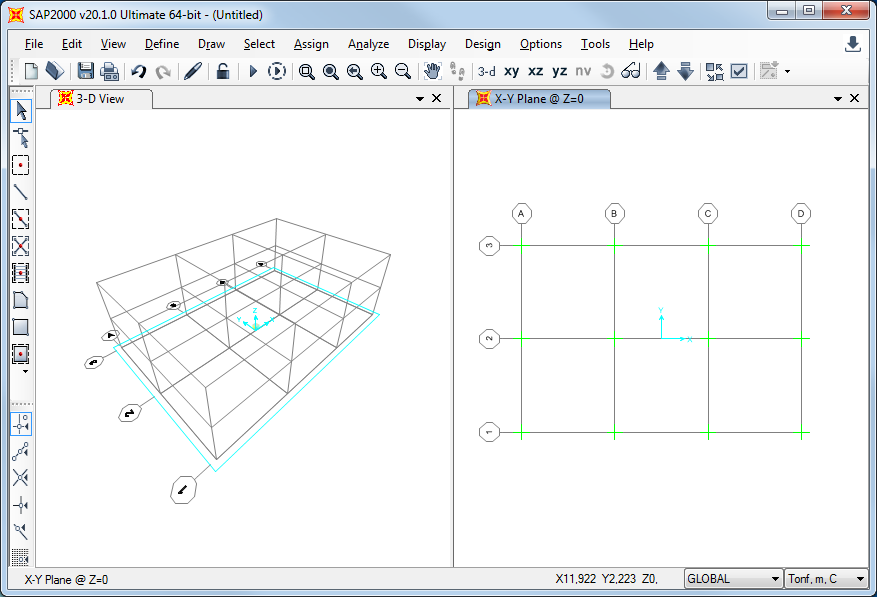
\includegraphics[width=1\textwidth]{metodologia/sap2000_axes.png}
%     \caption{Entorno virtual de SAP2000\textsuperscript{\textregistered} con un conjunto de ejes definido.}
%     \label{fig:sap2000_axes}
% \end{figure}

% Los menús del programa de computador que permiten ingresar los elementos del modelo consisten en aquellos que permiten escoger el tipo de elemento, como se muestra en la figura \ref{fig:sap200_draw}, y aquellos que permiten modificar los elementos ya ingresados, los cuales permiten moverlos, copiarlos, o eliminarlos. \\
% \begin{figure}[ht]
%     \centering
%     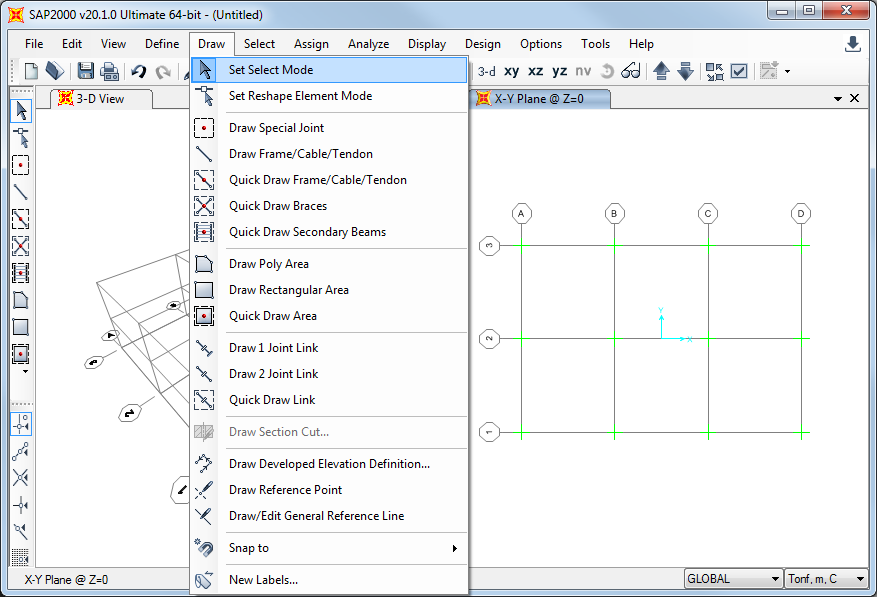
\includegraphics[width=1\textwidth]{metodologia/sap2000_draw.png}
%     \caption{Menú de SAP2000\textsuperscript{\textregistered} que permite ingresar diferentes tipos de elementos.}
%     \label{fig:sap200_draw}
% \end{figure}

% Una vez el usuario haya agregado los diferentes elementos de la estructura puede modificar sus condiciones de apoyo, las cargas, entre otros, mediante el uso de menús, de manera que el modelo esté listo para que el programa ejecute el análisis correspondiente. En la figura \ref{fig:sap2000_model} se presenta el modelo de una estructura terminado.
% \begin{figure}[ht]
%     \centering
%     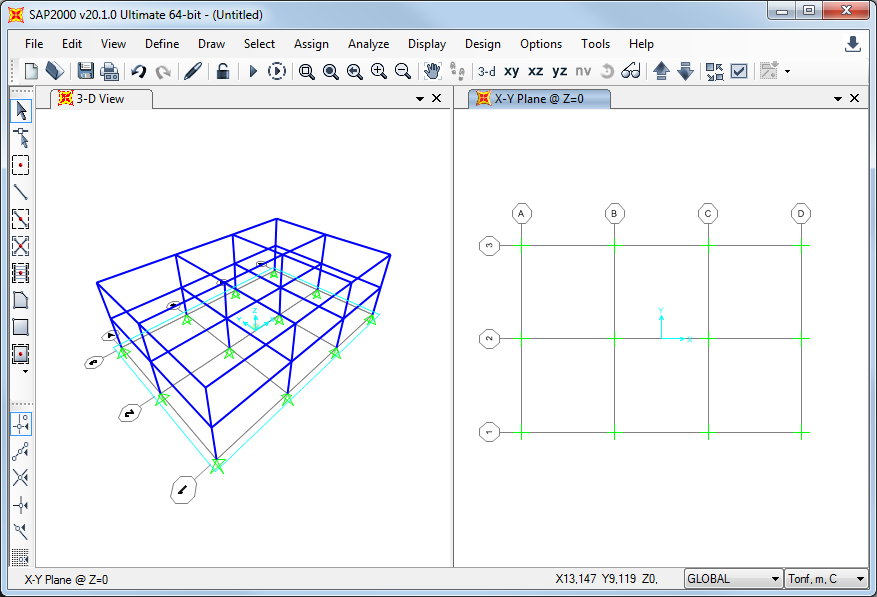
\includegraphics[width=1\textwidth]{metodologia/sap2000_model.png}
%     \caption{Modelo de una estructura en  SAP2000\textsuperscript{\textregistered}.}
%     \label{fig:sap2000_model}
% \end{figure}

% Una vez se han surtido los pasos anteriores, el usuario puede correr el análisis para obtener los resultados del mismo. El usuario puede visualizar los resultados en el entorno virtual, como se muestra en la figura \ref{fig:sap2000_deformed}, o mediante tablas.
% \begin{figure}[ht]
%     \centering
%     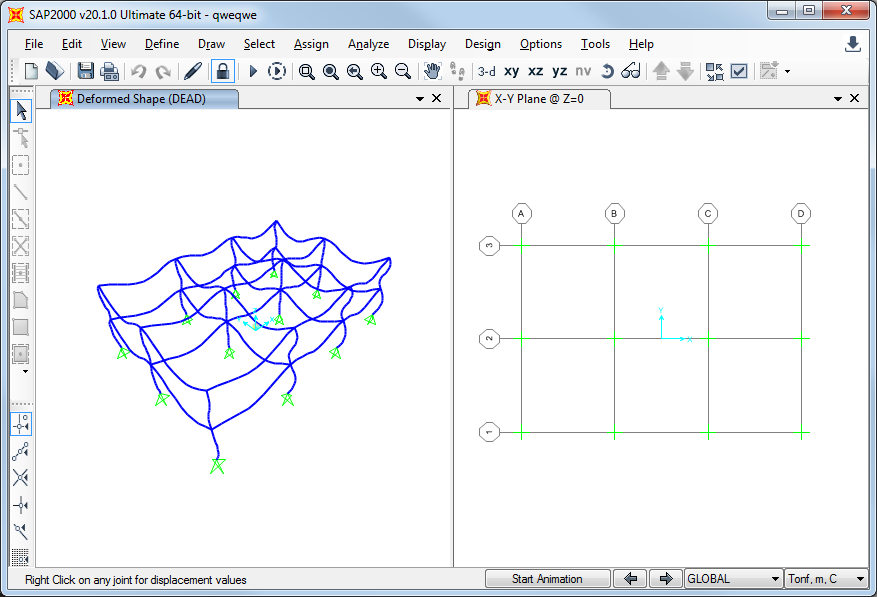
\includegraphics[width=1\textwidth]{metodologia/sap2000_deformed.png}
%     \caption{Deformación de la estructura después del análisis de SAP2000\textsuperscript{\textregistered}.}
%     \label{fig:sap2000_deformed}
% \end{figure}

% Así como el programa SAP2000\textsuperscript{\textregistered}, los otros programas comerciales, como ETABS \textsuperscript{\textregistered}, CSIBridge\textsuperscript{\textregistered}, midas\textsuperscript{\textregistered}, entre otros, cuentan con herramientas similares para que el usuario pueda analizar modelos de estructuras.

% \section{Revisión de los programas a código abierto}
% Existen gran variedad de programas a código abierto. Entre los programas que más se han estudiado para este trabajo se encuentra \textit{ANALEST}. \\

% El programa \textit{ANALEST} comprende una serie de subprogramas cuyo objeto es servir de ayuda en el análisis y diseño de estructuras. El programa está programado en \texttt{BASIC} y su característica principal es analizar 
% \begin{inparaenum}[$ (1) $]
%     \item vigas continúas, 
%     \item armaduras planas, 
%     \item armaduras en el espacio, 
%     \item pórticos planos, 
%     \item pórticos en el espacio, 
%     \item parrillas planas.
% \end{inparaenum}

% Para usar los subprogramas, se debe
% \begin{inparaenum}[$ (1) $]
%     \item introducir los datos del modelo de la estructura, revisarlos y guardarlos, 
%     \item introducir los datos de carga, revisarlos y guardarlos, 
%     \item ejecutar el análisis, guardar los resultados y presentarlos
% \end{inparaenum}

% Ademas, los subprogamas de vigas y armaduras permiten encontrar la envolvente de momentos en los apoyos y de fuerzas axiales, respectivamente, como paso preliminar para el diseño de los miembros. \\

% Guardar los datos estructurales y los datos de carga es muy útil en aquellos casos en que conviene modificar las dimensiones de los elementos con base en los resultados del primer análisis. Por otra parte, guardar los resultados facilita el estudio de las combinaciones de carga disminuyendo por una parte los datos requeridos y por otra el tiempo de ejecución, ya que se aprovecha el principio de superposición. Adicionalmente, guardar dichos resultados facilita el enlace de los subprogramas con programas de diseño, bien sean adquiridos o desarrollados por el usuario. \\

% \section{Identificación de los elementos a programar}

% De la revisión de los diferentes programas comerciales se dedujo que el programa StressUN debía dividirse en tres partes y que tenían que trabajar en conjunto. Dichas partes son: \textit{preproceso}, \textit{proceso} y \textit{posproceso}. \\

% El preproceso consiste en la adquisición de todos los datos relevantes del modelo de la estructura a analizar. El proceso realiza el tratamiento de los datos del modelo, mientras que el posproceso presenta los resultados del análisis del modelo. \\

% Tanto el preproceso como el posproceso necesitan de un ambiente gráfico, mientras que el proceso necesita de las rutinas propias del análisis matricial. \\

% \section{Selección de las herramientas de programación}
% Los dos grandes problemas a solucionar consistieron en desarrollar el ambiente gráfico, el cual se compone de menús y un entorno virtual tridimensional, y el núcleo de StressUN. Para esto, se consultó las diferentes herramientas de programación disponibles, donde se decidió utilizar la librería \textit{frames}, la cual está programada en el \textit{Java}, y el conjuto de librerías \textit{Scipy}, la cual está programada en \textit{Python}.\\

% La librería frames consiste en un conjunto de herramientas para crear un entorno virtual bidimensional o tridimensional interactivo. Dicha librería trabaja como una extensión de la librería \textit{processing}, la cual también está programada en Java. \\

% La librería processing es un conjunto de herramientas dirigida a solucionar los problemas relacionados con la computación gráfica, permitiendo a los desarrolladores desde crear imágenes hasta entornos virtuales tridimensionales. \\

% Por otro lado, el conjunto de librerías Scipy consiste en herramientas para solucionar problemas relacionados algebra matricial. Dicho conjunto de librerías está conformado por \textit{Numpy}, \textit{Scipy}, \textit{matplotlib}, entre otros. La librería Numpy provee arreglos multidimensionales y operaciones entre ellos. La librería \textit{Scipy} trata problemas del algebra matricial, como son la solución de sistemas de ecuaciones líneales, mientras que matplotlib permite generar diferentes tipos de gráficos. \\

% \section{Desarrollo del programa de computador}

% Una vez se identificaron los diferentes elementos necesarios con los que debía contar el programa de computador y se escogieron las herramientas de trabajo, se realizó una revisión bibliográfica de la formulación matemática de los métodos matriciales aplicados al análisis estructural, enfocada al análisis de estructuras tridimensionales de respuesta lineal. Adicionalmente, se realizó una revisión a la documentación de la librería frames.\\

% De dicho ejercicio se identificaron los datos de entrada que el usuario necesita definir y los datos de salida que espera obtener
% \begin{itemize}
%     \item \textit{Preproceso}
%     \begin{itemize}
%         \item Definición de los materiales.
%         \item Definición de las secciones transversales.
%         \item Definición de los nudos.
%         \item Definición de los elementos.
%         \item Definición de las condiciones de apoyo.
%         \item Definición de los casos de carga.
%         \item Definición de las combinaciones de carga.
%         \item Definición de las patrones de carga
%     \end{itemize}
%     \item \textit{Posproceso}
%     \begin{itemize}
%         \item Visualización de los desplazamientos en los nudos.
%         \item Visualización de las reacciones.
%         \item Visualización de las fuerzas internas.
%     \end{itemize}
    
% \end{itemize}

%  \textit{StressUN} se desarrolló usando el paradigma de \textit{programación orientada a objetos}, \textit{OOP} (de sus siglas en inglés \textit{object-oriented programming}), y en forma modular, de manera que el \textit{preproceso} y el \textit{posproceso} son independientes del \textit{proceso}.\\

% A medida que se definieron los diferentes elementos a tener en cuenta, se fueron programando. Es decir, se desarrollaron las clases \textit{primitivas} del programa, las cuales representan la abstracción de los elementos de las entidades más sencillas del problema, las cuales consisten en las clases
% \begin{itemize}
%     \item \textit{Material}.
%     \item \textit{Section}.
%     \item \textit{Node}.
%     \item \textit{Frame}.
%     \item \textit{Support}.
%     \item \textit{PointLoad}.
%     \item \textit{LoadPattern}.
%     \item \textit{Displacement}.
% \end{itemize}

% Las clases anteriormente listadas, tienen su representación tanto en el preproceso y posproceso, como en el proceso. Es decir, en el preproceso y posproceso dichas clases tienen su representación gráfica, mientras que en el proceso, éstos tienen su representación matemática. Sin embargo, dichas clases son separadas unas de las otras, de manera que se asegure que el preproceso y posproceso son independientes del proceso.

% Una vez programados las entidades más básicas del programa, se procedió a crear la clase \textit{Structure}, la cual se encarga de administrar otros objetos. Dicho paradigma de programación se conoce como \textit{composición}. Los objetos que contiene la clase \textit{Structure} son

% \begin{itemize}
%     \item \textit{Materials}.
%     \item \textit{Sections}.
%     \item \textit{Nodes}.
%     \item \textit{Frames}.
%     \item \textit{Supports}.
%     \item \textit{LoadPatterns}.
% \end{itemize}

% Cada una de las anteriores clases es la interfaz entre el programa y el usuario, donde este último podrá agregar nuevos materiales, secciones, nudos, elementos tipo pórtico, condiciones de apoyo y condiciones de carga. Dichas clases componen el \textit{núcleo} del programa.\\

% El proceso anteriormente descrito se desarrolló bajo los diferentes mecanismos que provee la programación orientada objeto, los cuales son encapsulación, herencia y sobre carga. Estas herramientas, bien aplicadas, permiten la reutilización del código y el mantenimiento del mismo. Así mismo, se utilizó la herramienta de \textit{Git}, la cual es un sistema de control de versiones, la cual permite llevar el control absoluto durante el proceso de desarrollo del código.\\

% \section{Verificación del programa}

% Una vez se llegó a una versión estable del programa, este se puso a prueba mediante la solución de diferentes problemas que aparecen en la bibliografía, donde se comparó la respuesta obtenida con la presentada. Así mismo, se comparó el desempeño del programa frente a otros programas, tanto comerciales como académicos, en cuanto a la facilidad de uso como al tiempo de computo. \\
